\documentclass{article}
\usepackage[utf8]{inputenc}
\usepackage{graphicx}
\usepackage{tikz}
\usepackage{listings}
\usepackage{float}
\usepackage{amsmath}
\usetikzlibrary{positioning,fit,calc,arrows.meta, shapes}
\graphicspath{ {images/} }

%Tot això hauria d'anar en un pkg, però no sé com és fa

\newcommand*{\assignatura}[1]{\gdef\1assignatura{#1}}
\newcommand*{\grup}[1]{\gdef\3grup{#1}}
\newcommand*{\professorat}[1]{\gdef\4professorat{#1}}
\renewcommand{\title}[1]{\gdef\5title{#1}}
\renewcommand{\author}[1]{\gdef\6author{#1}}
\renewcommand{\date}[1]{\gdef\7date{#1}}
\renewcommand{\maketitle}{ %fa el maketitle de nou
    \begin{titlepage}
        \raggedright{UNIVERSITAT DE LLEIDA \\
            Escola Politècnica Superior \\
            Grau en Enginyeria Informàtica\\
            \1assignatura\\}
            \vspace{5cm}
            \centering\huge{\5title \\}
            \vspace{3cm}
            \large{\6author} \\
            \normalsize{\3grup}
            \vfill
            Professorat : \4professorat \\
            Data : \7date
\end{titlepage}}
%Emplenar a partir d'aquí per a fer el títol : no se com es fa el package
%S'han de renombrar totes, inclús date, si un camp es deixa en blanc no apareix

\tikzset{
	%Style of nodes. Si poses aquí un estil es pot reutilitzar més facilment
	pag/.style = {circle, draw=black,
                           minimum width=0.75cm, font=\ttfamily,
                           text centered},
	base/.style = {rectangle, rounded corners, draw=black,
                           minimum width=4cm, minimum height=1cm,
                           text centered}
}
\renewcommand{\figurename}{Figura}
\renewcommand{\tablename}{Taula}

\title{Xarxes - Pràctica 1}
\author{Sergi Simón Balcells\\21040111X}
\date{Diumenge 7 de Abril}
\assignatura{Xarxes}
\professorat{Enric Guitart, Carles Mateu}
\grup{GM3}

%Comença el document
\begin{document}
\maketitle
\thispagestyle{empty}

\newpage
\pagenumbering{roman}
\tableofcontents
\newpage
\pagenumbering{arabic}

\section{Introducció}
%1. L’estructura, a nivell esquemàtic (diagrama de blocs), del client i del servidor.
%2. L’estratègia emprada per el manteniment de la comunicació, tant en el client com en el servidor.
%3. Un diagrama d’estats del protocol implementat sobre UDP (registre i manteniment de la comunicació).
%4. Totes aquelles consideracions que cregueu oportunes
\section{Estructura}
\subsection{Estructura del client}
\begin{figure}[h]
	\centering
	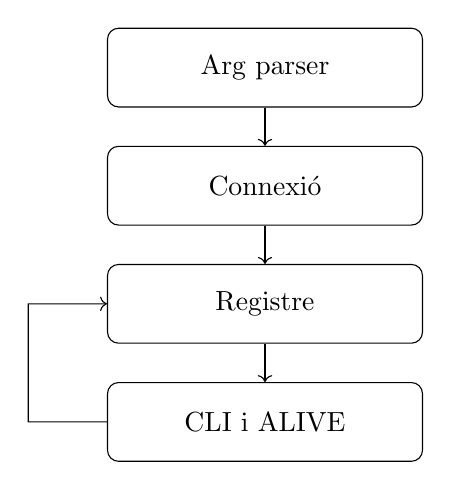
\begin{tikzpicture}[node distance=1.5cm]
		\node (arg) [base]               {Arg parser};
		\node (con) [base, below of=arg] {Connexió};
		\node (reg) [base, below of=con] {Registre};
		\node (cal) [base, below of=reg] {CLI i ALIVE};
		
		\draw[->] (arg) -- (con);
		\draw[->] (con) -- (reg);
		\draw[->] (reg) -- (cal);
		\draw[->] (cal.west) -- ++(-1, 0) -- ++(0, 1.5) -- (reg.west);
	\end{tikzpicture}
	\label{est:cli}
	\caption{Estructura principal del client mitjançant un diagrama de blocs}
\end{figure}
\subsection{Estructura del Servidor}
\begin{figure}[h]
	\centering
	\begin{tikzpicture}[node distance=1.5cm]
		\node (arg) [base] 				 {Arg parser};
		\node (con) [base, below of=arg] {Connexió};
		\node (clt) [base, below of=con] {Clients};
		\node (man) [base, below of=clt] {Manager i ALIVE UPDATE};
		
		\draw[->] (arg) -- (con);
		\draw[->] (con) -- (clt);
		\draw[->] (reg) -- (man);
	\end{tikzpicture}
	\label{est:ser}
	\caption{Estructura principal del servidor mitjançant un diagrama de blocs}
\end{figure}
\begin{figure}[h]
	\centering
	\begin{tikzpicture}[node distance=1.5cm]
		\node (sel) [base] 				 {Select de stdin, socket udp i tcp};
		\node (thr) [base, below of=arg] {Thread amb objectiu del tipus};
		\node (tra) [base, below of=con] {Tractament del input};
		
		\draw[->] (sel) -- (thr);
		\draw[->] (thr.west) -- ++(-1, 0) -- ++(0, 1.5) -- (sel.west);
		\draw[->, dashed] (thr) -- (tra);
	\end{tikzpicture}
	\label{est:man}
	\caption{Estructura del mànager del servidor}
\end{figure}
\section{Estratègia}
En aquesta secció es parlarà sobre les estratègies utilitzades per a mantenir la 
connexió, és a dir, la fase d'alives tant del servidor com del client.\\
\\
\subsection{Estratègia client}
En el client, mitjançant un procés aïllat d'atendre la línia de comandes,
s'efectuarà periodicacment un enviament d'alive al al servidor, una espera
de R segons i un select no bloquejant per veure si hi ha hagut contestació en
aquest període. Si hi ha hagut contestació per part del servidor es tracta
aquesta resposta. En el cas que sigui un ALIVE\_ACK amb tots els camps correctes,
es reiniciarà el comptador del client d'alives, el qual a cada volta del bucle
es baixarà en un. Si aquest contador arriba a 0, es dona per perduda la connexió
amb el servidor, tallant la interfície de comandes i tornant a començar un nou
procés de registre.\\
\\
% Afegir diagrama sobre l'estrategia d'alive fase.
\subsection{Estratègia servidor}
En el servidor s'utilitzaran dos fils. En el primer fil, cada $0,5s$ es baixarà 
un comptador d'alives de tots els clients, sempre i quan el seu estat sigui 
diferent a desconnectat. Aquest procés simula una TTL (time to live) amb uns quants
pasos més, ja que identifica l'estat dels clients.\\
\\
En l'altre fil atenc totes les peticions que li poden arribar al servidor, com es mostra
en la figura \ref{est:man}. En el cas concret de mantindre la connexió, quan rep un
paquet ALIVE\_INF, evalua l'estat del paquet, i, en cas de tenir la PDU correcte, envia
un ALIVE\_ACK i restaura el valor del comptador d'alives de la taula.\\
\\
% Diagrama de l'estrategia del servidor
\section{Diagrama d'estats}
\section{Consideracions}
% Comentar tests -t 2 i -t 4 en el servidor
% Comentar -d <nombre> del client i el motiu
% Deamon en el servidor
\end{document}






















